\def\ArtHome[#1]{{\tt <ARTISYNTH\_HOME>#1}}

\title{ArtiSynth Installation Guide for \SYSTEM{}}
\author{John Lloyd, Sebastian Kazenbroot-Guppy, and Antonio S{\'a}nchez}
\setpubdate{Last updated: March, 2018}
\iflatexml
\date{}
\fi

\newif\ifNeedLibraryPath
\NeedLibraryPathfalse

\begin{document}

\maketitle

\iflatexml{\large\pubdate}\fi

\tableofcontents

\section{Introduction}

This document describes how to install and run ArtiSynth
on \FULLSYSTEM{} machines. There are two ways to obtain ArtiSynth:
downloading a prepackaged release, or cloning the latest development
version from Github. Downloading a prepackaged release is the easiest
solution to simply try out some of the basic demo programs. Cloning
the development version is recommended for developers who want to keep
their codebase current.

The typical install sequence looks like this:

\begin{description}

\item[Download]\mbox{}

Download either a release (Section \ref{PrepackagedRelease}) or
checkout (i.e., {\it clone}) out the development version
(Section \ref{GitClone}).

\item[Build]\mbox{}

Compile the system (Section \ref{Building}). This
step is not needed for prepackaged releases.

\item[Run]\mbox{}

Start ArtiSynth and run the demonstration models (Section \ref{Running}).

\end{description}

Generally, users will also want to install and run external models and
packages that have been created either by others or by themselves.
This is discussed in (Section \ref{AdditionalModelsAndPackages}).

\section{Prerequisites}

To install ArtiSynth on \SYSTEM{}, you will need:

\begin{itemize}

\item A 64 bit version of \SYSTEM{}

\item Java 8

\item Linux systems require GNU libc version 2.17 or higher

\item A three button mouse is recommended for GUI interaction

\end{itemize}

Note that we have stopped officially supporting 32 bit systems, both
because they are becoming obsolete, and because ArtiSynth applications
often require more memory than they can provide.

For Java, the full Java development kit (JDK) is required, which comes
with the Java compiler {\tt javac}. The run time environment (JRE)
will not be sufficient. However, there is no need for extra bundles
such at JavaFX, NetBeans, or EE.

At the time of this writing, JDKs can be obtained free from Oracle at
\begin{quote}
\href{http://www.oracle.com/technetwork/java/javase/downloads/index.html}%
{http://www.oracle.com/technetwork/java/javase/downloads/index.html}.
\end{quote}
We recommend obtaining a JDK for Java 8, for which the latest update
is Java SE 8u162.

\begin{sideblock}
By default, ArtiSynth is compiled to be compliant with Java 8. While
it should also be possible to run ArtiSynth under Java 9, there have
been reports of compatibility problems and warnings involving the Java
OpenGL (JOGL) interface. Therefore we recommend using Java 8 until
these issues are resolved. Java 8 is also compatible with current
releases of MATLAB, which is useful if one wishes to run ArtiSynth
from MATLAB.
\end{sideblock}

\begin{sideblock}
Java versions 5 and earlier had an additional ``1.'' prepended to
their number, so that Java 5 was called 1.5. This numbering scheme
still persists informally, so that Java 8 is occasionally referred to
as 1.8, etc.
\end{sideblock}
 
In this document, the location of the ArtiSynth installation \directory{}
will be denoted by \ArtHome[]. for example
if ArtiSynth is installed in
\ifWindows
\begin{verbatim}
  C:\people\roger\artisynth_core
\end{verbatim}
then \ArtHome[] denotes this \directory{}
and \ArtHome[\SEP lib] denotes the sub-\directory{}
\begin{verbatim}
  C:\people\roger\artisynth_core\lib
\end{verbatim}
\else
\begin{verbatim}
  /home/roger/artisynth_core
\end{verbatim}
then \ArtHome[] denotes this \directory{}
and \ArtHome[\SEP lib] denotes the sub-\directory{}
\begin{verbatim}
  /home/roger/artisynth_core/lib
\end{verbatim}
\fi

\section{Downloading a Prepacked Release}
\label{PrepackagedRelease}

\subsection{Downloading and unpacking the zip file}

To obtain one of the packaged distributions, go to
\href{http://www.artisynth.org/downloads}%
{www.artisynth.org/downloads}
and select the distribution
you want. Download it, and unzip it in an appropriate location on your
computer.

\ifWindows
\begin{sideblock}
{\bf Important:}\\
On \SYSTEM{}, it is highly recommended that ArtiSynth is not installed
in a location for which any of the \directory{} names contain spaces (i.e.,
{\tt Program Files}).  This can be important for some ArtiSynth
programs to run correctly.
\end{sideblock}
\else\fi

Once ArtiSynth is downloaded and unpacked, it should be possible to
run it immediately by executing the
\ifWindows
{\tt artisynth.bat} file located in \ArtHome[\SEP bin]
(see Section \ref{artisynthBat}).
\else
{\tt artisynth} command located in \ArtHome[\SEP bin]
(see Section \ref{artisynthCommandLine}).
\fi

\section{Cloning from Github}
\label{GitClone}

Github is a web-based repository service based on the source control
management system Git. A very brief summary of Git is given in
Section \ref{GitSummary}.

The latest ArtiSynth development version is available from Github at the URL
\begin{verbatim}
   https://github.com/artisynth/artisynth_core.git
\end{verbatim}
Users can checkout (i.e., clone) this version and then continue to
update their codebase to keep it current
(Section \ref{UpdatingArtiSynth}). 
In some casess, developers we work closely with can also obtain, by
mutual arrangement, write access to our Github repository, allowing
them to also commit changes.

\begin{sideblock}
Users who have a Github account combined with SSH keys may instead
wish to clone using the SSH URL
\begin{verbatim}
   git@github.com:artisynth/artisynth_core.git
\end{verbatim}
For users with repository write access, this will allow them to
perform subsequent {\tt push} operations without having to
enter a username and password.
\end{sideblock}

\subsection{Cloning the repository}

There are several ways to clone ArtiSynth from Github.

\ifWindows

\subsubsection{Clone using Git for Windows}
\label{CloningUsingGitForWindows}

Install Git for Windows (Section \ref{GitForWindows}), and then from
either Git Bash or the {\tt CMD} console, enter the command
%
\begin{lstlisting}[]
  git clone https://github.com/artisynth/artisynth_core.git [<dir>]
\end{lstlisting}
%
The argument {\tt <dir>} is optional and gives the name of the
\directory{} into which the repository and working copy should be
extracted; if omitted, the \directory{} will be named {\tt
artisynth\_core}.

\subsubsection{Cloning using Cygwin}

If you have Cygwin (Section \ref{Cygwin}) installed, along with the
{\tt git} package, then you can check out ArtiSynth within a Cygwin
shell window using the same {\tt git clone} command described
in Section \ref{CloningUsingGitForWindows}.

\else
\subsubsection{Cloning using the command line}

Assuming your \SYSTEM{} distribution has Git installed, then you can
clone ArtiSynth from Github using the following command:
%
\begin{lstlisting}[]
 > git clone https://github.com/artisynth/artisynth_core.git [<dir>]
\end{lstlisting}
%
The argument {\tt <dir>} is optional and gives the name of the
\directory{} into which the repository and working copy should be
extracted; if omitted, the \directory{} will be named {\tt
artisynth\_core}.
\fi

\subsubsection{Cloning using Eclipse}
\label{ArtiSynthEclipseCheckout}

If you are planning to develop ArtiSynth models in Java, and if you
are planning to do this with the Eclipse IDE
(Section \ref{EclipseIDE}), then it might be easier to do the Git
clone directly in Eclipse.  Follow the instructions in
Section \ref{importingFromGit}, using the URL {\tt
https://github.com/artisynth/artisynth\_core.git} described above.

\subsection{Downloading the libraries}
\label{DownloadingLibraries}

Because the {\tt jar} files and native libraries used by ArtiSynth
are large, they are not stored in the Github repository.
Instead, they must be downloaded separately. This can be
done using the command \updateArtisynthLibs, located
in \ArtHome[\SEP bin].
\ifWindows
You can execute it by double-clicking on it in a file-browser, or
by opening a command console ({\tt CMD}), navigating
to \ArtHome[], and entering the command
\begin{verbatim}
 % bin\updateArtisynthLibs
\end{verbatim}
\else
You can execute it from the command line like this:
\begin{verbatim}
 > cd <ARTISYNTH_HOME>
 > bin/updateArtisynthLibs
\end{verbatim}
\fi

\ifWindows
If you have Cygwin (Section \ref{Cygwin}) installed, 
the same command is available as {\tt
updateArtisynthLibs}, also located in \ArtHome[\SEP bin].
\else\fi

\section{Building ArtiSynth}
\label{Building}

If ArtiSynth has been cloned from Github, it will be necessary to
build (compile) it. 

If ArtiSynth was obtained as a prepackaged release, then it is
precompiled and does not need to be built in order to run the built-in
demos. However, it will generally be useful to build ArtiSynth anyway,
particularly since any user-defined models created in Java will
themselves need to be compiled.

Java compilation and code development is typically done using an
integrated development environment (IDE), although it is possible
(particularly on Linux and MacOS) to use external text editors and
command line tools. This document describes how to build and run
ArtiSynth using either the Eclipse IDE, or
\ifWindows
command line tools available in the Cygwin Unix emulator.
\else
shell-based command line tools.
\fi
For more information on Eclipse, see Section \ref{EclipseIDE}.

\subsection{Building with Eclipse}
\label{BuildingWithEclipse}

If your Github clone has been done externally to Eclipse (i.e.,
not according to Section \ref{ArtiSynthEclipseCheckout}), then you
need to first import ArtiSynth into Eclipse. Follow the instructions
in Section \ref{importingExternalProjects}.

Once ArtiSynth has been imported, you should be able to build it.  If
necessary, first open a Java perspective by choosing {\sf Window >
Open Perspective > Java}. The project {\tt artisynth\_core} (or
whatever you might have named it) should appear in the {\sf Package
Explorer} window. To build the system, select the project in the {\sf
Package Explorer} window, and then choose {\sf Project > Build
Project}. Note that it may be necessary to deselect {\sf Build
Automatically} in order to enable {\sf Build Project}.

\ifWindows
\subsection{Building with Cygwin}
\label{BuildingWithCygwin}

If you have Cygwin (Section \ref{Cygwin}) installed, 
ArtiSynth can also be built from a Cygwin terminal by running
a {\tt make} command in the top level \directory{}. Before doing this,
you need to first set the environment variables {\tt ARTISYNTH\_HOME}
and {\tt CLASSPATH} as described in Sections
\ref{EnvironmentVariables} and \ref{CygwinEnvironmentSettings}.
ArtiSynth can then be built by executing

\begin{verbatim}
 > cd <ARTISYNTH_HOME>
 > make
\end{verbatim}
\else
\subsection{Building from the command line}
\label{BuildingWithCygwin}

ArtiSynth can also be built by running a {\tt make} command in the top
level \directory{}. Before doing this, you need to first set the environment
variables {\tt ARTISYNTH\_HOME} and {\tt CLASSPATH} as described in
Sections \ref{EnvironmentVariables}. ArtiSynth can then be built by
executing

\begin{verbatim}
 > cd <ARTISYNTH_HOME>
 > make
\end{verbatim}
\fi

\section{Running ArtiSynth}
\label{Running}

\ifWindows
\subsection{Running using artisynth.bat}
\label{artisynthBat}

The most direct way to start ArtiSynth is to run the batch file
{\tt artisynth.bat}, located in \ArtHome[\SEP bin].  This can be
done by double-clicking on it in a file browser.

You can also create a shortcut to this batch file (by right clicking
on it and selecting {\sf Create Shortcut}), and then placing this shortcut
in either the {\sf START} menu or on the Desktop. However, the batch file
itself must remain in \ArtHome[\SEP bin].

Alternatively, you can open a command console ({\tt CMD}), navigate
to \ArtHome[], and enter the command
%
\begin{verbatim}
 % bin\artisynth
\end{verbatim}
%
It is recommended to place \ArtHome[\SEP bin] 
in your {\tt PATH} environment variable (Section \ref{EnvironmentVariables}),
so that the console command simplifies to
\begin{verbatim}
 % artisynth
\end{verbatim}
regardless of the current directory.

\begin{sideblock}
{\bf Note:}\\
If Java is installed in a non-conventional location, the system may
not be able to find it and this will cause {\tt artisynth.bat} to fail.
To fix this, locate the \directory{} in which {\tt java.exe} resides, and let
the location of this \directory{} be called JAVA\_DIR. You should then add
JAVA\_DIR to your system's {\tt PATH} environment variable (see
Section \ref{settingWindowsPath}).  
\end{sideblock}

\subsection{Running using Cygwin}

If you have Cygwin (Section \ref{Cygwin}) installed, 
then you can run ArtiSynth directly with the {\tt artisynth} command
located in \ArtHome[/bin]:
\begin{verbatim}
 > cd <ARTISYNTH_HOME>
 > bin/artisynth
\end{verbatim}
If \ArtHome[/bin] has been placed in your {\tt PATH}
variable (Section \ref{EnvironmentVariables}), then it
is sufficient to do
\begin{verbatim}
 > artisynth
\end{verbatim}
{\tt artisynth} can be called with a number of options; to see these, run
\begin{verbatim}
 > artisynth -help
\end{verbatim}

\else
\subsection{Running from the command line}
\label{artisynthCommandLine}

The most direct way to start ArtiSynth is to run the command
\ArtHome[\SEP bin\SEP artisynth]:
%
\begin{verbatim}
 > cd <ARTISYNTH_HOME>
 > bin/artisynth
\end{verbatim}
It is recommended to place \ArtHome[/bin] in your {\tt PATH}
environment variable (Section \ref{EnvironmentVariables}), so
that the command simplifies to
\begin{verbatim}
 > artisynth
\end{verbatim}
regardless of the current directory.

\ifMacOS
\subsection{Running from the file browser}

You can also run ArtiSynth from a file browser by double clicking on
\begin{verbatim}
  <ARTISYNTH_HOME>/bin/artisynth.command
\end{verbatim}
Note that {\tt artisynth.command} is just a copy of {\tt artisynth};
the {\tt .command} suffix makes it recognizable to the MacOS GUI as a
command.
\fi\fi

\subsection{Command line arguments}
\label{CommandLineArguments}

The {\tt artisynth} command accepts command line arguments, a full
list of which can be seen by running {\tt artisynth} with the {\tt
-help} option:
\ifWindows
\begin{verbatim}
 % artisynth -help
\end{verbatim}
\else
\begin{verbatim}
 > artisynth -help
\end{verbatim}
\fi
Descriptions of these options appear in various places within the
ArtiSynth documentation. For example, one commonly used option is
{\tt -model <modelClassName>}, which instructs ArtiSynth to preload a
model associated with a given class name:
\ifWindows
\begin{verbatim}
 % artisynth -model artisynth.demos.mech.SpringMeshDemo
\end{verbatim}
\else
\begin{verbatim}
 > artisynth -model artisynth.demos.mech.SpringMeshDemo
\end{verbatim}
\fi

\subsection{Running using Eclipse}

Once ArtiSynth has been imported into Eclipse (and built if
necessary), it should contain a launch configuration called {\tt
ArtiSynth} that will allow ArtiSynth to be run by choosing {\sf Run >
Run}.

In some cases, one may wish to adjust environment variables, command
line arguments, or Java JVM arguments to affect how ArtiSynth behaves.
Instructions for doing so are contained in Sections
\ref{EclipseEnvironmentVariables} and \ref{EclipseCommandArguments}.

\subsection{Loading and Running Models}

Once ArtiSynth starts up, you can use it to load and run
models. General instructions on how to load and run models are given
in the section ``Loading and Simulating Models'' of the
\artisynthManual{uiguide}{ArtiSynth User Interface Guide}. 

By default, ArtiSynth comes with a number of demonstration models,
which can be loaded and run as follows:

From the menu bar, Select {\sf Models > Demos}.  This will display a
submenu of demonstration models. Choosing one will cause that model to
be loaded and displayed in the viewer.  Simulation of the model can
then be started, paused, single-stepped, or reset using the play
controls (Figure \ref{PlayControlsFig}) located at the upper right of
the ArtiSynth window frame.

\begin{figure}
\begin{center}
\iflatexml
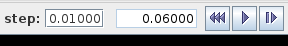
\includegraphics[]{images/playControls}
\else
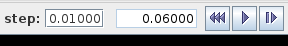
\includegraphics[width=2.5in]{images/playControls}
\fi
\end{center}
\caption{The ArtiSynth play controls. From left to right: step size
control, current simulation time, and the reset, play/pause, and
single-step buttons.}%
\label{PlayControlsFig}
\end{figure}

Comprehensive information on exploring and interacting with models is
given in the
\artisynthManual{uiguide}{ArtiSynth User Interface Guide}.

\section{Installing External Models and Packages}
\label{AdditionalModelsAndPackages}

Typically, an ArtiSynth developer will want to use external models and
packages that exist outside of {\tt artisynth\_core}.  Some of these
may be obtained from external sources.  For example, {\tt
artisynth\_models} is a collection of packages that provides a variety
of publicly available anatomical models, currently focussed primarily
on the head and neck region. For instructions on obtaining {\tt
artisynth\_models}, visit 
\href{https://www.artisynth.org/models}{www.artisynth.org/models}.

Installing external models and packages requires a sequence of
operations similar to that for installing ArtiSynth itself:

\begin{enumerate}

\item Download

\item Build (if necessary)

\item Run

\end{enumerate}

\subsection{Downloading}

Some model and package collections, such as {\tt artisynth\_models}
mentioned above, may be available either as prepackaged distributions,
or through Git or Subversion repositories.  Prepackaged distributions
should be downloaded and unpacked into a desired location, while Git
or Subversion checkouts may may be obtained as described in
Sections \ref{GitSummary} or \ref{SubversionSummary}.

Some collections maintained by ArtiSynth may contain Eclipse project
settings (in an {\tt eclipseSettings.zip} file in their root
\directory{}), allowing them to be imported into Eclipse, either
directly from Git (Section \ref{importingFromGit}) or Subversion (
Section \ref{importingFromSubversion}),
or after being obtained separately 
(Section \ref{importingExternalProjects}).

\subsection{Building}

Collections that are obtained from Git or Subversion will need to be
built (compiled).

\subsubsection{Building with Eclipse}

Many collections (such as {\tt artisynth\_models}) can be imported
into Eclipse as a project and then built as described in Section
\ref{BuildingWithEclipse}.

\begin{sideblock}
Important: for collection projects to compile properly in Eclipse, the
{\tt artisynth\_core} project (and any other projects they depend on)
will have to be added to their build path. The default Eclipse
settings supplied with some projects (in the file {\tt
eclipseSettings.zip}) may already contain the required build path
dependencies. For example, the settings for {\tt artisynth\_models}
contain the required reference to {\tt artisynth\_core}.  In other
cases, it may be necessry to add projects to the build path
explicitly, as described in \ref{AddingProjectsToBuildPath}.
\end{sideblock}

\subsubsection{Building from the command line}

If the collection has a {\tt Makefile} in its root
\directory{}, then it can be compiled from
\ifWindows
a Cygwin terminal by running {\tt make} in the root \directory{}. 
\else
the command line by running {\tt make} in the root \directory{}.
\fi
Before doing this, the top-level directory for the collection's {\tt
class} files must to be added to the {\tt CLASSPATH} environment
variable
\ifWindows
(Sections \ref{EnvironmentVariables} and \ref{CygwinEnvironmentSettings}).
\else
(Section \ref{EnvironmentVariables}).
\fi
In collections maintained by ArtiSynth, this will be the directory {\tt
classes}, located directly under the collection root directory (e.g.,
{\tt artisynth\_models\SEP classes}).

\subsection{Running}

External models are executed by running ArtiSynth itself (Section
\ref{Running}). However, in order to execute these models, ArtiSynth
must be able to locate their associated classes. This can be
arranged in three different ways:

\subsubsection{Adding external classes using the Eclipse Classpath}

If you are running from Eclipse, then you can make the classes of
external projects visible to ArtiSynth by adding the projects to the
{\sf Classpath} of your ArtiSynth launch configuration, as described
in Section \ref{AddingProjectsToLaunch}.

\subsubsection{Adding external classes using EXTCLASSPATH}

Alternatively, you can make the classes of external projects visible
to ArtiSynth by adding the path names of all their top-level class
\directories{} (or {\tt jar} files, if relevant) to the file 
\ArtHome[\SEP EXTCLASSPATH] (described in Section
\ref{EXTCLASSPATHFile}).

For example, suppose the collection {\tt artisynth\_models}
has been placed in {\tt \TOP projects\SEP artisynth\_models}.
The top-level class \directory{} for this collection is located
in {\tt artisynth\_models\SEP classes}, and so the following entry
should be placed in the {\tt EXTCLASSPATH} file:

\ifWindows
\begin{verbatim}
C:\projects\artisynth_models\classes
\end{verbatim}
\else
\begin{verbatim}
/projects/artisynth_models/classes
\end{verbatim}
\fi

\subsubsection{Adding external classes using CLASSPATH}

\ifWindows
Finally, if you are running using {\tt artisynth.bat} (or {\tt
artisynth} in Cygwin), then you can make external classes visible by
adding them to your {\tt CLASSPATH} environment variable (see Sections
\ref{EnvironmentVariables} and \ref{CygwinEnvironmentSettings}).
\else
Finally, if you are running from the command line using the {\tt
artisynth} command, then you can make external classes visible by adding
them to your {\tt CLASSPATH} environment variable (see Section
\ref{EnvironmentVariables}).
\fi

\section{Updating ArtiSynth}
\label{UpdatingArtiSynth}

One reason to use a clone of the latest ArtiSynth
development version is to be able to migrate recent changes into your
code base. When a significant update occurs, a posting is made to the
ArtiSynth update log, currently located at
\artisynthManual{updates}{www.artisynth.org/doc/html/updates/updates.html}.
Users may also be notified via the {\tt artisynth-updates} email list.

Users working from Eclipse may update simply by selecting
the project in the {\sf Package Explorer} and selecting {\sf Team >
Pull} from the context menu.

\ifWindows
Updating may also be done by issuing the 
\begin{verbatim}
   > git pull
\end{verbatim}
command from within the ArtiSynth installation \directory{}, 
using either Git for Windows (Section \ref{GitForWindows}),
the Cygwin shell (Section \ref{Cygwin}), or another Git application.
\else
Updating may also be done from the command line by issuing the 
\begin{verbatim}
   > git pull
\end{verbatim}
command from within the ArtiSynth installation \directory{}.
\fi

\subsection{Library updates}

Occasionally, a software update will be accompanied by a change in the
libraries located in \ArtHome[\SEP libs].  When this
happens, it will be indicated on the ArtiSynth update log and
appropriate instructions will be given. Sometimes, it will be
necessary to explicitly update the libraries after doing the main
update. This can be done by executing {\tt updateArtisynthLibs} as
described in Section \ref{DownloadingLibraries}.

\section{The Eclipse IDE}
\label{EclipseIDE}

Eclipse is an integrated development environment (IDE) commonly used
for Java code development, and many ArtiSynth developers use it for
both developing models in Java and for running the system. This section
describes how to load ArtiSynth projects into Eclipse, and how to
configure it for running ArtiSynth. A general introduction to Eclipse
is beyond the scope of this document, but there are many Eclipse
resources available online.

\subsection{Obtaining Eclipse}

Eclipse can be obtained from
\href{http://www.eclipse.org/downloads}{www.eclipse.org/downloads}.  A
good version to obtain (at the time of this writing) is {\sf Eclipse
IDE for Java Developers}.

\begin{sideblock}
The Eclipse instructions described below are based on the ``Neon''
distribution, but should be largely similar for later versions.
\end{sideblock}

\subsection{Importing ArtiSynth projects into Eclipse}

ArtiSynth projects include the core distribution ({\tt
artisynth\_core}), the open source models collection {\tt
artisynth\_models} (which contains human anatomy models), as well as
other model and code collections maintained by the ArtiSynth team and
other users.

There are several ways to import ArtiSynth projects into Eclipse.  If
the project has already been downloaded or checked out from a
repository, then it can be imported as an external project
(Section \ref{importingExternalProjects}). Otherwise, Eclipse itself
can be used to check out a project from either Git
(Section \ref{importingFromGit}) or Subversion
(Section \ref{importingFromSubversion}).

\subsubsection{Importing external projects}
\label{importingExternalProjects}

ArtiSynth project repositories (including {\tt artisynth\_core} and
{\tt artisynth\_models}) do {\it not} directly expose the Eclipse
project files ({\tt .project}, {\tt .classpath}, etc.) within the
distribution. Instead, these files are bundled within a top-level file
{\tt eclipseSettings.zip}, which must be unzipped directly into the
top-level \directory{}, as described in Section
\ref{installingProjectFiles}. This is to prevent local modifications to the
project files from being propagated back to the main
repositories. 

Let {\tt <PROJECT\_DIR>} denote the top-level project \directory{}.  For the
core distribution {\tt artisynth\_core}, this will also be
\ArtHome[].

\begin{enumerate}

\item From {\bf outside} Eclipse, extract the Eclispe project files by
unzipping {\tt <PROJECT\_DIR>\SEP eclipse\-Settings.zip} into {\tt
<PROJECT\_DIR>}.
\ifMacOS
MacOS users are strongly encouraged to read  
Section \ref{installingProjectFiles} for details on how to do this.
\else
For details, see Section \ref{installingProjectFiles}.
\fi

\ifMacOS
\begin{sideblock}
{\bf Attention MacOS users:}\\[0.5em]
The default zip utility on MacOS will create a new sub-folder called 
{\tt eclipseSettings} and will extract the files there.  
\emph{You do not want this!!}
Some of the files are then labeled as ``hidden'' by MacOS, which will
prevent you from moving them to the correct place manually. 
Either extract the file directly to the \ArtHome[] directory 
with a more standard application like {\sf 7-Zip} ({\sf 7zX} for OSX), 
or use the {\tt unzip} utility from the command-line.  For the latter,
open a terminal window, change to the ArtiSynth install directory,
and enter the command
\begin{verbatim}
  unzip eclipseSettings.zip
\end{verbatim}
\end{sideblock}
\fi

\item For {\tt artisynth\_core}, then from {\bf outside} Eclipse, 
download the required {\tt jar} files and native libraries as
described in Section \ref{DownloadingLibraries}.

\item From within Eclipse, choose {\sf File > Import ...}.

\item An {\sf Import} dialog will appear. 
Select {\sf General > Existing Projects into Workspace} and click {\sf Next}.

\item An {\sf Import Projects} dialog will appear. 
In the field {\sf Select root directory}, enter (or browse to) the
{\it parent} \directory{} of {\tt <PROJECT\_DIR>}. The project
itself should now appear in the {\sf Projects} box (Figure
\ref{EclipseImportProjects:fig}). (If other projects are contained in the 
parent directory, these will appear as well.)
Make sure that the
desired project is selected and then click {\sf Finish}.

\end{enumerate}

\begin{sideblock}
If Eclipse complains that {\sf "No projects are found to import"}, or
does not otherwise show the project as available for import,
then most likely the {\tt <PROJECT\_DIR>}
\directory{} does not contain a {\tt .project} file. This 
can happen if {\tt eclipseSettings.zip} was not properly unzipped into
{\tt <PROJECT\_DIR>}.
\end{sideblock}

\begin{figure}
\begin{center}
\iflatexml
   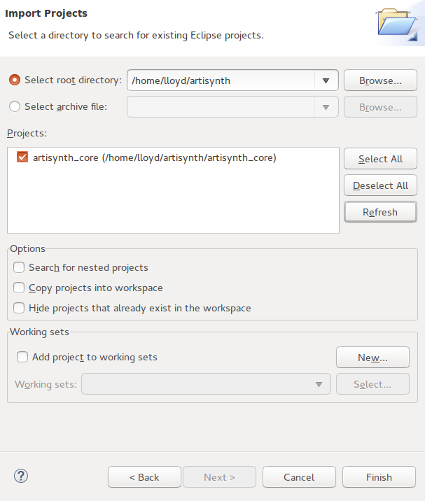
\includegraphics{images/EclipseImportProjectsLinuxSmall}
\else
   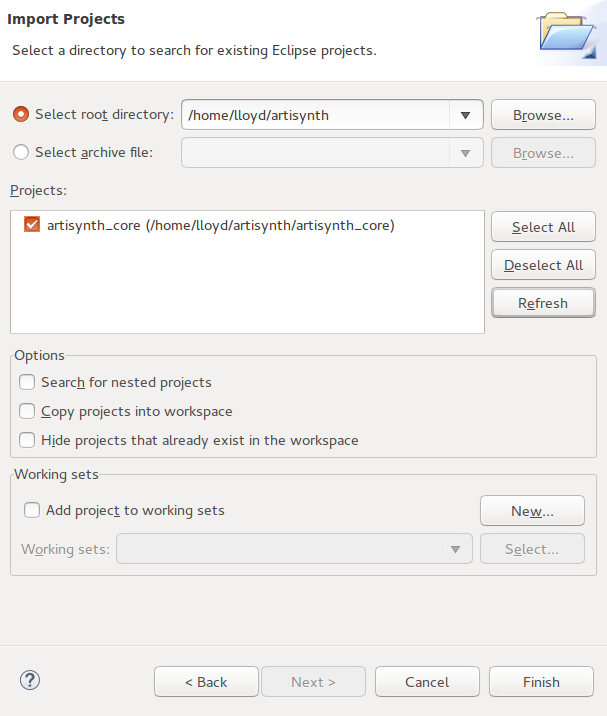
\includegraphics[width=0.4\textwidth]{images/EclipseImportProjectsLinux}
\fi   
\end{center}
\caption{Eclipse Import Projects dialog.}%
\label{EclipseImportProjects:fig}
\end{figure}

\subsubsection{Importing from a Git repository}
\label{importingFromGit}

Recent versions of Eclipse contain integrated support for Git, and so
importing a project directly from a Git repository is relatively easy.

Because ArtiSynth GIT repositories do not directly expose Eclipse
project files, the standard import method of
%
\begin{quote}
{\sf File > Import... > Git > Projects from Git}
\end{quote}
%
will not work completely. Instead, one must
first clone the Git repository, and then import the
project \directory{} as described in
Section \ref{importingExternalProjects}.

To clone a Git repository from within Eclipse;

\begin{enumerate}

\item Choose {\sf Window > Show View > Other ... > Git > Git Repositories} 
from the main menu to open a {\sf Git Repositories} view window.

\item Within the {\sf Git Repositories} window, choose the
button (or pull down menu item) that says {\sf Clone a repository}.

\item 
A {\sf Source Git Repository} dialog will appear (Figure
\ref{EclipseGitImport:fig}, left). Enter the URL for the
repository. For ArtiSynth itself, this is {\tt
https://github.com/artisynth/artisynth\_core.git}).  The {\sf URI}
field is coupled to some of the others: you can either fill in the
{\sf URI} field directly, or enter the individual URI components in
the {\sf Host}, {\sf Repository path}, and {\sf Protocol} fields.
Also, if the repository has read access restrictions, it will
generally be necessary to specify a user name and password in the {\sf
Authentication} fields.  After entering the required information,
click {\sf Next}. 

\item A {\sf Branch Selection} dialog may appear. If it does,
select only the {\sf master} branch, and then click {\sf Next}.

\item A {\sf Local Destination} dialog will appear (Figure
\ref{EclipseGitImport:fig}, right). In the {\sf Directory} field, enter
the path of the local \directory{}, which will contain both the cloned
repository and the working copy.  For ArtiSynth itself, this will also
be the ArtiSynth home \directory{} (\ArtHome[]).  After
entering the \directory{} information, click {\sf Finish}.

\end{enumerate}

Finally, import the local \directory{} into Eclipse as a project by
following the steps in Section \ref{importingExternalProjects}, using the
local \directory{} parent as the ``root directory''.

\begin{figure}
\begin{center}
\begin{tabular}{cc}
\iflatexml
   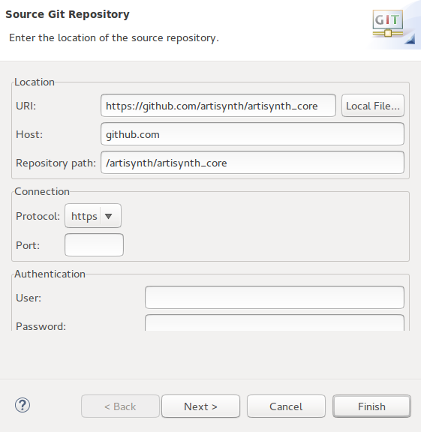
\includegraphics{images/EclipseSourceGitRepositorySmall} &
   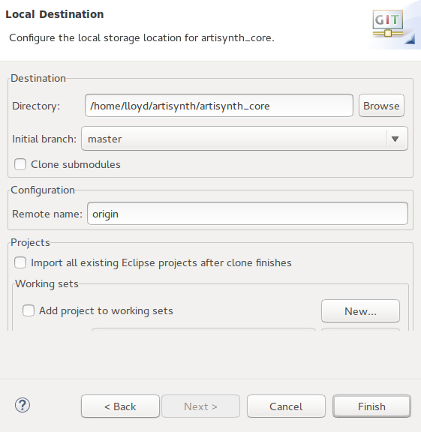
\includegraphics{images/EclipseLocalDestinationSmall}
\else
   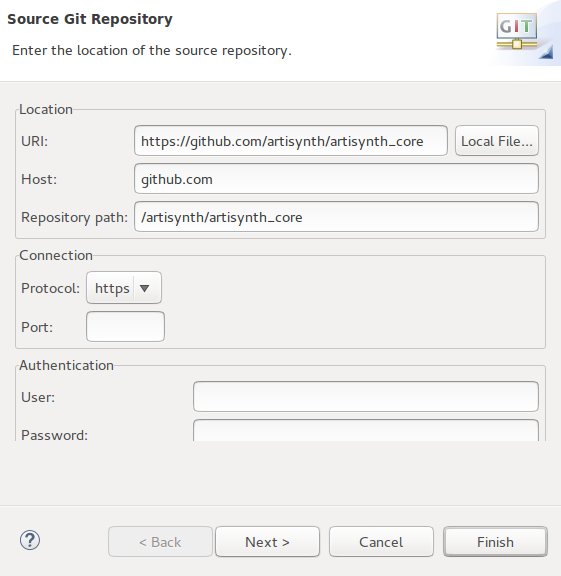
\includegraphics[width=0.45\textwidth]{images/EclipseSourceGitRepository} &
   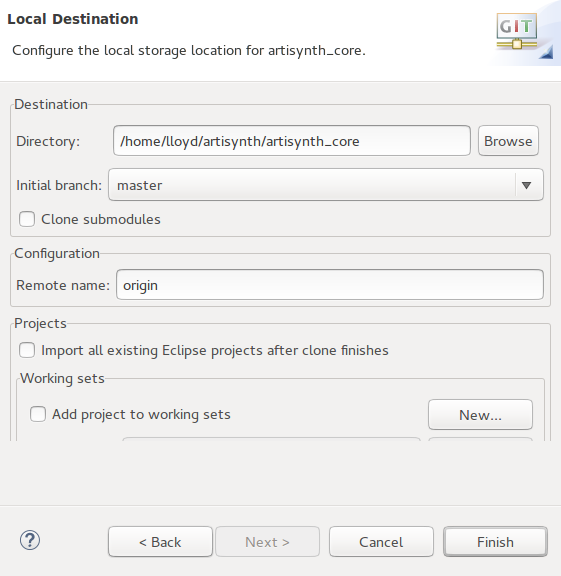
\includegraphics[width=0.45\textwidth]{images/EclipseLocalDestination}
\fi   
\end{tabular}
\end{center}
\caption{Eclipse dialogs for importing a Git repository.}%
\label{EclipseGitImport:fig}
\end{figure}

\subsubsection{Importing from a Subversion repository}
\label{importingFromSubversion}

If Eclipse has a Subversion plug-in installed (Section
\ref{SubversionPlugIn}), you may import an ArtiSynth project by
checking it out directly from the repository located by
the project's {\it Subversion\_URL}. For the core ArtiSynth
distribution, this is 
\begin{verbatim}
   https://svn.artisynth.org/svn/artisynth_core/trunk
\end{verbatim}
Other projects will have different URLs.

The following instructions assume the Subversive plug-in.

\begin{enumerate}

\item Choose {\sf File > Import} from the main menu, select {\sf SVN >
Project from SVN} and click {\sf Next}.

\item You now need to specify a repository location, as specified by a
{\it Subversion\_URL}.  If you've previously done an SVN checkout, a
menu will appear allowing you to select a previously used URL. If one
of these is sufficient, select it and click {\sf Next} to go to Step
4. Otherwise, select {\sf Create a new repository location} and click
{\sf Next} to enter a repository dialog. If no previous locations are
known this dialog will appear automatically.

\item If you are specifying a new location in the repository dialog:

\begin{itemize}

\item Under the {\sf General} tab, enter the {\it Subversion\_URL} in the
{\sf URL} box. If you are just checking out the trunk of the
repository (i.e., if your Subversion URL ends in {\tt /trunk}), then
you should omit the final {\tt /trunk} since this is selectable in Step 4.

\item If you are checking out a repository that is not available for
anonymous access, or if you need write access to the repository, enter
your ArtiSynth User ID and Password (which you will have obtained from
us separately) in the {\sf Authentication} section of the dialog.
You will probably want to check {\sf Save authentication} as well.

%\item If you are just checking out the trunk of the repository (i.e.,
%if your Subversion URL ends in {\tt /trunk}, as most examples in this
%guide do), then go to the {\sf Advanced} tab and uncheck {\sf Enable
%Structure Detection}.

\item Click {\sf Next}.

\end{itemize}

\item In the {\sf Select Resource} dialog, use the {\sf URL} selector
box to select the full URL to be used for the checkout. If you are
just checking out the trunk of the repository, then choose {\tt
Subversion\_URL/trunk} which should be available as a selection.

\item Click {\sf Finish}

\item In the {\sf Check Out As} dialog, select {\sf Check out as a
project with name specified}, adjust the project name if desired,
and click {\sf Next}.

\item Specify the location for the check out. If you leave {\sf Use
default workspace location} selected, this will be {\tt
workspace/project\_name}, where {\tt workspace} is the Eclipse
workspace \directory{} and {\tt project\_name} is the project name
selected in the previous step. Otherwise, you can specify an explicit
checkout location (which does not have to be located in the Eclipse
workspace). For ArtiSynth core checkouts, the project name is
typically {\tt artisynth\_core} and the the checkout location will
become the ArtiSynth install \directory{} \ArtHome[].

\item Click {\sf Finish}.

\item If necessary, open a Java perspective by choosing {\sf Window >
Open Perspective > Java}. The project should appear in the {\sf
Package Explorer} window.

\item From {\bf outside} Eclipse, install the Eclipse project files by
unzipping {\tt <PROJECT\_DIR>\SEP eclipse\-Settings.zip} into {\tt
<PROJECT\_DIR>}. 
\ifMacOS
MacOS users are strongly encouraged to read  
Section \ref{installingProjectFiles} for details on how to do this.
\else
For details, see Section \ref{installingProjectFiles}.
\fi

\item From {\bf outside} Eclipse, download
the required {\tt jar}
files and native libraries as described in Section \ref{DownloadingLibraries}.

\item Finally, load the new settings into the project by selecting the
project in the {\sf Package Explore} window and selecting {\sf
Refresh} from the context menu.

\end{enumerate}

\subsubsection{Installing project files}
\label{installingProjectFiles}

Distributions of {\tt artisynth\_core} and {\tt artisynth\_models}, as
well as some other project repositories, contain their eclipse project
files bundled in the zip file {\tt eclipseSettings.zip}.  The reason
for not placing project files directly under repository control is to
prevent local changes to them from being propagated back into the
repository.

Let {\tt <PROJECT\_DIR>} denote the top-level project \directory{}.
%
\ifWindows
On Windows, project files can be extracted from within the 
file browser. Double click on {\tt eclipseSettings.zip}
and extract the files into {\tt <PROJECT\_DIR>}.
\else
Project files can be extracted using the command line.
Open a command shell, 
switch to the {\tt <PROJECT\_DIR>} \directory{}, and run {\tt unzip}:
\begin{verbatim}
  > cd <PROJECT_ROOT>
  > unzip eclipseSettings.zip
\end{verbatim}
\fi
This will create the files {\tt .project} and {\tt .classpath}, along
with the \directory{} {\tt .settings}, in {\tt <PROJECT\_DIR>}.  In
the case of {\tt artisynth\_core}, it will also create the file {\tt
ArtiSynth.launch} containing the default launch configuration.

\begin{sideblock}
Note: if unzip queries about overwriting {\tt .project}, answer [y]es.
\end{sideblock}

\ifMacOS
\begin{sideblock}
{\bf Attention MacOS users:}\\[0.5em]
While it is possible to unzip files from the file browser by clicking
on {\tt eclipseSettings.zip} and then extracting directly, the default
zip utility on MacOS will create a new sub-folder called {\tt
eclipseSettings} and will extract the files there.
\emph{You do not want this!!}
Some of the files are then labeled as ``hidden'' by MacOS, which will
prevent you from moving them to the correct place manually. 
Either extract the files using the command line as described
above, or use a more standard application like {\sf 7-Zip} ({\sf 7zX} for OSX).
\end{sideblock}
\fi

\subsection{Configuring environment variables}
\label{EclipseEnvironmentVariables}

When running ArtiSynth from Eclipse, it may be useful to set certain
environment variables that affect its operation.  Directions on
setting the environment variables are given in
Section \ref{SettingEnvironmentVariables}, and descriptions of the
variables themselves may be found in
Section \ref{EnvironmentVariables}.

Some variables that are commonly set within Eclipse include:

\begin{itemize}

\item {\tt ARTISYNTH\_HOME}: If set, this should be set to
\ArtHome[]. Normally ArtiSynth is able to infer its own location
internally, so it is generally unecessary to set this variable
explictly.

\item {\tt OMP\_NUM\_THREADS}: Specifies the maximum number of processor cores
available for multicore execution.

\item {\tt ARTISYNTH\_PATH}: A list of folders, separated by semi-colons ";", 
which ArtiSynth uses to search for configuration files. 
See Section \ref{EnvironmentVariables}.

\end{itemize}

If any of the above variables have already been set externally in
\SYSTEM{} (\environmentSectionRef), such that they are visible
to Eclipse at start-up, then they do not need to be set in the launch
configuration.

%In addition to setting environment variables, if you are running Java
%1.7 (but not Java 1.8), then you should increase the memory space
%allocated for classes. Do this by adding the following JVM argument to
%your launch configuration:
%%
%\begin{lstlisting}
% -XX:MaxPermSize=100M
%\end{lstlisting}
%%
%Instructions for doing this are given in Section
%\ref{SettingCommandLineArguments}.

\ifNeedLibraryPath

\begin{sideblock}
{\bf Important:} At present, eclipse does not expand environment variables.
In all the variable settings described below, references to 
\ArtHome[]should be expanded (manually) to the path of the
ArtiSynth install \directory{}.
\end{sideblock}

\ifWindows
\begin{sideblock}
{\bf Note:} There is a bug in Eclipse 4.0+ on Windows where it will replace 
the system's native {\tt \%PATH\%} variable rather than appending to it.  
To correct this behavior, define {\tt PATH} as 
{\tt \$\{env\_var:path\};\$ARTISYNTH\_HOME\SEP lib\SEP \ARCH{}} 
\end{sideblock}
\fi
\fi

\subsubsection {Setting environment variables}
\label{SettingEnvironmentVariables}

To set environment variables within Eclipse:

\begin{enumerate}

\item Open a java perspective if necessary by choosing
  {\sf Window > Open Perspective > Java}.

\item Select the ArtiSynth project in the {\sf Package Explorer} form.

\item Choose {\sf Run > Run Configurations...} to open the {\sf Run
  Configurations} window.

\item In the left panel, under {\sf Java Application}, select {\sf ArtiSynth}.

\item In the right panel, select the {\sf Environment} tab.

\item To create a new environment variable, click the {\sf New} button and
  enter the name and value in the dialog box. 
See Figure \ref{EclipseEnvVariables:fig}.

\item When finished, make sure that {\sf Append environment to native
  environment} is selected, and click {\sf Apply}.

\end{enumerate}

\begin{figure}
\begin{center}
\iflatexml
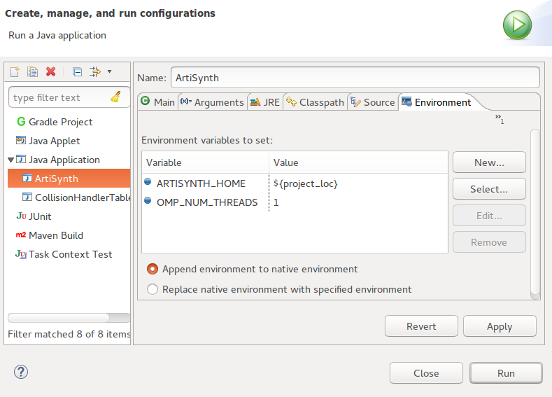
\includegraphics[]{images/EclipseEnvVariablesSmall}
\else
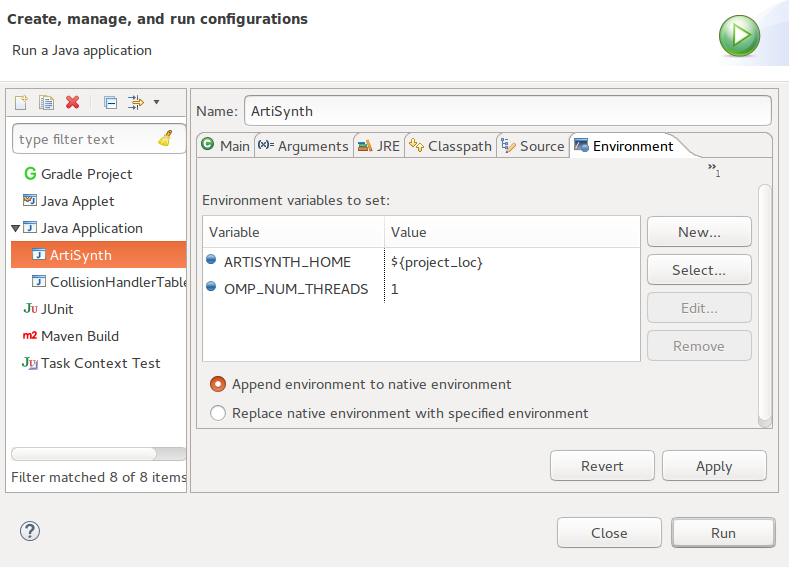
\includegraphics[width=5.0in]{images/EclipseEnvVariables}
\fi
\end{center}
\caption{Setting environment variables within Eclipse.}%
\label{EclipseEnvVariables:fig}
\end{figure}

\subsection{Command line and JVM arguments}
\label{EclipseCommandArguments}

As described in Section \ref{CommandLineArguments}, the {\tt artisynth}
command accepts command line arguments. To invoke these when
running from Eclipse, it is necessary to set the desired arguments in
the launch configuration, as described below. 

Sometimes it may also be necessary to set JVM arguments, which control
the Java virtual machine running ArtiSynth.  An example of such an
argument is {\tt -Xmx}, which can be used to increase the maximum
amount of memory available to the application.  For example, {\tt
-Xmx6g} sets the maximum amount of memory to 6 gigabytes.

\subsubsection {Setting command line and JVM arguments}
\label{SettingCommandLineArguments}

To set command line arguments for your Eclipse application:

\begin{enumerate}

\item Open a java perspective if necessary by choosing
  {\sf Window > Open Perspective > Java}.

\item Select the ArtiSynth project in the {\sf Package Explorer} form.

\item Choose {\sf Run > Run Configurations...} to open the {\sf Run
  Configurations} window.

\item In the left panel, under {\sf Java Application}, select {\sf ArtiSynth}.

\item In the right panel, select the {\sf Arguments} tab.

\item Program arguments (which are passed directly to ArtiSynth)
should be specified in the {\sf Program arguments} box.  JVM arguments
should be specified in the {\sf VM arguments} box. See Figure
\ref{EclipseRunArguments:fig}.

\item When finished, click {\sf Close}.

\end{enumerate}

\begin{figure}
\begin{center}
\iflatexml
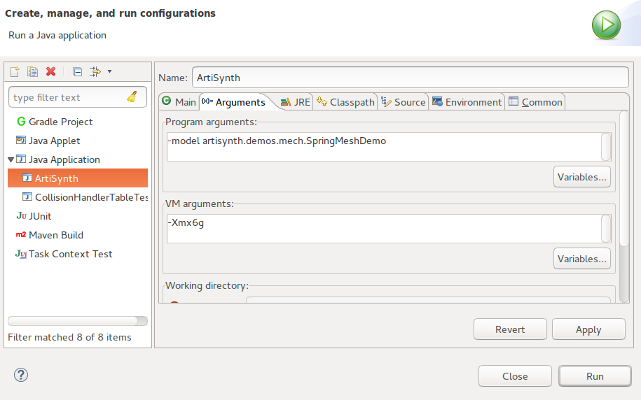
\includegraphics[]{images/EclipseRunArgumentsSmall}
\else
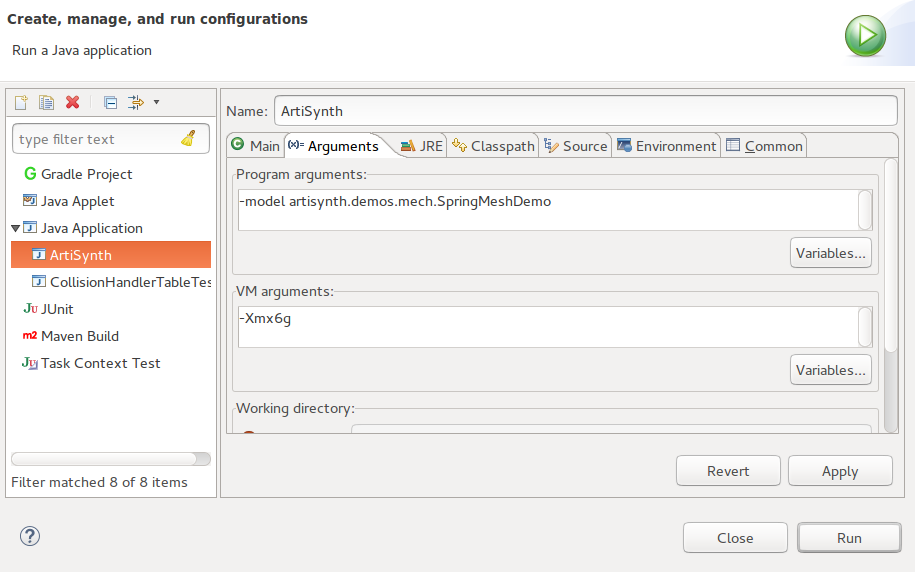
\includegraphics[width=5.0in]{images/EclipseRunArguments}
\fi
\end{center}
\caption{Setting command line and JVM arguments for a run configuration.}%
\label{EclipseRunArguments:fig}
\end{figure}


\subsection{Adding projects to the build path}
\label{AddingProjectsToBuildPath}

A project imported into Eclipse may depend on the packages and
libraries found in other projects to compile properly.  For example,
ArtiSynth applications which are external to {\tt artisynth\_core}
will nonetheless depend on {\tt artisynth\_core}. To ensure proper
compilation, project dependencies should be added to each dependent
project's build path.

\begin{enumerate}

\item Select the dependent project in the {\sf Package Explorer} form.

\item Right click and choose {\sf Build Path > Configure Build Path...} 

\item In the right panel, select the {\sf Projects} tab.

\item Click the {\sf Add} button, select the project dependencies,
      and click {\sf OK}

\item Click {\sf OK} in the Java Build Path panel

\end{enumerate}

\subsection{Adding projects to the ArtiSynth launch configuration}
\label{AddingProjectsToLaunch}

The classes of external projects can be made visible to ArtiSynth by
adding the projects to the Classpath of the ArtiSynth launch
configuration.

\begin{enumerate}

\item From the main menu, choose {\sf Run > Run Configurations...}
to open a {\sf Run Configurations} dialog.

\item In the left panel, under {\sf Java Application}, select your
ArtiSynth launch configuration (the default one is called {\sf
ArtiSynth}). This may already be selected when you open the panel.

\item In the right panel, select the {\sf Classpath} tab.

\item In the {\sf Classpath:} window, select {\sf User Entries},
and then click the {\sf Add Projects} button.

\item In the {\sf Project Selection} dialog, select the external
projects that you wish to add. Generally, the boxes
{\sf Add exported entries ...} and {\sf Add required projects ...}
can be unchecked. Click {\sf OK}.

\item Close the {\sf Run Configurations} dialog.

\end{enumerate}

\subsection{Installing a Subversion plug-in}
\label{SubversionPlugIn}

In order to work with Subversion from within Eclipse, either to check
out ArtiSynth from the repository, or to update or commit changes, it
is necessary to use a Subversion plug-in. First, check to see if your
version of Eclipse contains an Subversion plug-in:

Open an import panel using {\sf File > Import...}, and then look for
{\sf SVN} in the set of available import sources. If you don't see SVN
listed, it will be necessary to install a plug-in.

We recommend the Eclipse-supported Subversive plug-in, but if this
proves difficult for any reason, there are other options, such as
Subclipse, currently obtainable from
\href{http://subclipse.tigris.org/servlets/ProjectProcess?pageID=p4wYuA}%
{subclipse.tigris.org}.

Instructions for installing Subversive can be obtained at
\href{http://www.eclipse.org/subversive/installation-instructions.php}%
{www.eclipse.org/subversive/installation-instructions.php}.

One way to install Subversive is through the Eclipse Marketplace.  If
you have an older version of Eclipse that doesn't have Marketplace,
you may be able to obtain it from
\href{http://www.eclipse.org/mpc/}{www.eclipse.org/mpc}.  To access
the Marketplace, click {\sf Help > Eclipse Marketplace}. Once the
available applications have been displayed, type {\tt Subversive} into
the {\sf Find} box in the top-left corner of the Marketplace
window. Navigate to the package labeled {\sf Subversive - SVN Team
Provider} and click {\sf Install}. On the {\sf Confirm Selected
Features} screen, ensure all boxes are checked and click the button
labeled {\sf Confirm >}. Restart Eclipse when prompted.

One more step is now necessary. Re-open Eclipse, and you should be
prompted to choose an SVN connector in the start menu.  SVN connectors
interface Subversive to the SVN server, and are OS and
server-specific. A recommended SVN Connector will be pre-selected for
downloading; this is most likely the one you need.

If Eclipse did not prompt you to choose a connector when it restarted,
you can install SVN connectors separately (thanks to bmaupin at
Stackoverflow for this information):

\begin{enumerate}

\item  Go to 
\href{http://www.polarion.com/products/svn/subversive/download.php}%
{www.polarion.com/products/svn/subversive/download.php}

\item Under the latest {\sf Release}, copy the Subversive SVN
Connectors URL. The current URL for Eclipse 4.3 Kepler
is \href{http://community.polarion.com/projects/subversive/download/eclipse/3.0/kepler-site/}%
{http://community.polarion.com/projects/subversive/download/eclipse/3.0/kepler-site}.

\item In Eclipse, go to {\sf Help > Install New Software...} and 
click {\sf Add...}  

\item Copy the URL for the Subversive SVN Connectors into the {\sf
Location} box and click {\sf OK}

\item Check {\sf Subversive SVN Connectors}, click {\sf Next}, and
then follow the instructions to complete installation.

\end{enumerate}

If in doubt about the connector you need, you can install multiple
ones, and then adjust the one Subversive actually uses by going to
{\sf Windows > Preferences}, opening {\sf Team > SVN}, and then
opening the {\sf SVN Connector} tab.

\subsection{Preventing excessive resource copying}

By default, ArtiSynth classes are built in a directory tree ({\tt
<PROJECT\_DIR>\SEP classes}) that is separate from the source tree ({\tt
<PROJECT\_DIR>\SEP src}), where {\tt <PROJECT\_DIR>} denotes the project
root \directory{} and is \ArtHome[] for ArtiSynth itself.
That means that Eclipse will try to copy all non-Java files and
\directories{} from the source tree into the build tree. For ArtiSynth,
this is excessive, and results in many files being copied that don't
need to be, since ArtiSynth looks for resources in the source tree
anyway.

It is possible to inhibit most of this copying:

\begin{enumerate}

\item Choose {\sf Window > Preferences} (or {\sf Eclipse > Preferences}).

\item Select {\sf Java > Compiler > Building}.

\item Open {\sf Output folder}, and in the box entitled {\sf Filter resources},
  enter the string:

\ifWindows
\begin{lstlisting}[]
    Makefile,*.a*,*.b*,*.c,*.cc,*.cxx,*.e*,*.g*,*.h*,*.i*,*.m*,*.n*,*.o*,*.r*,*.s*,*.t*
\end{lstlisting}
\else
\begin{lstlisting}[]
    Makefile,*.l*,*.?,*.??,*.???,*.????,???,????,?????
\end{lstlisting}
\fi

\end{enumerate}

That should filter out the copying of most non-java files.

Or, to prevent copying any resource, simply enter: 
\begin{lstlisting}[]
    *
\end{lstlisting}

\section{Additional Information}

\ifWindows

\subsection{Git for Windows}
\label{GitForWindows}

A version of Git for Windows can be installed from
\href{https://git-scm.com/download}{git-scm.com/download}.

It installs a version of Git Bash for that can be used for entering
Git commands.  While going through the install steps, there is an
option to select between:

\begin{enumerate}

\item Use Git from Git Bash only
\item Use Git from the Windows Command Prompt
\item Use Git and optional Unix tools from the Windows Command Prompt

\end{enumerate}

Option 2 (Git from CMD) is often fine for most users, and allows them
to run all git commands directly from a command console {\tt CMD}.  There are
other options for setting the default editor, the default
console to open when starting Git Bash, etc., but the defaults should
work well in most cases.

\subsection{The TortoiseSVN Client}
\label{TortoiseSVN}

As mentioned above, some ArtiSynth models may be distributed via
Subversion (SVN), and access to these will require an SVN client
program. A popular SVN client for Windows is TortoiseSVN, which can be
acquired from
\href{http://tortoisesvn.net}{tortoisesvn.net}. On that website,
navigate to {\sf Downloads} and then select the package appropriate
for your operating system (which presumably will be 64-bits).

Once downloaded, run the MSI installer and follow the instructions in
the installer. When the download completes, right-clicking in any file
browser in Windows should now present you with SVN version control
options, analogous to the command line instructions discussed in other
parts of the documentation. We will briefly discuss here the three
most common operations:

\begin{description}

\item[Checking out a repository]

To check out an SVN repository with TortoiseSVN, right-click in any
file exploration window and select {\sf SVN Checkout...} from the
context menu. The current directory will be the default directory for
the {\sf Checkout directory} field, and the {\it Subversion\_URL} can
be selected in the {\sf URL of repository} field. It is recommended
that other fields remain as their default values.

\item[Updating a working copy]

While inside a working copy of a repository in a file browser window,
updating that repository is as simple as right-clicking and selecting
{\sf SVN Update}.

\item[Committing changes]

Users which have write-access to a Subversion repository may commit
changes that they have made.  Right-click in a file browser window
inside a working copy of a repository and select {\sf
Commit...}. Write a commit message and the select {\sf OK}.

\end{description}

\subsection{Cygwin}
\label{Cygwin}

Cygwin provides Windows users with a Linux-like, shell-based command
environment.  Its provides useful tools and enables ArtiSynth users to
employ all the script-based commands in \ArtHome[\SEP bin], as well
as various {\tt Makefile} commands.

Cygwin can be downloaded from 
\href{http://www.cygwin.com}{www.cygwin.com}. Run the
executable that was just downloaded (setup.exe) to begin
installation. After selecting a download source, an install directory,
a package directory, an internet connection, and a download site, the
installer will display a list of packages which the user can select
for download. Normally, a default set of packages is already selected
for installation. It is advisable to install these packages to ensure
that Cygwin retains its basic capabilities. It is also recommended
that you select the following additional packages:

\begin{itemize}

\item {\tt archive}
\item {\tt git}, {\tt svn}, {\tt make} (located under {\tt devel})
\item {\tt python} (located under {\tt interpreters}).
\item {\tt openssh} (located under {\tt net})

\end{itemize}

If you are planning to compile C/C++ code, you may also want to
install the various {\tt gcc} and {\tt gdb} packages (located under {\tt devel}).
\fi

\subsection{Environment variables}
\label{EnvironmentVariables}

This is a glossary of all the environment variables that are
associated with building or running ArtiSynth. Often, the system can
detect and set appropriate values for these automatically. In other
cases, as noted in the above documentation, it may be necessary or
desirable for the user to set them explicitly.

\begin{description}

\item[ARTISYNTH\_HOME]\mbox{}
 
The path name of the ArtiSynth installation \directory{}.

\item[ARTISYNTH\_PATH]\mbox{}

A list of \directories{}, separated by \separatorDesc, which ArtiSynth
uses to search for configuration files such as {\tt .artisyntInit} or
{\tt .demoModels}.  A typical setting for {\tt ARTISYNTH\_PATH}
consists of the current \directory{} (indicated by "{\tt .}"), the user's
home \directory{}, and the ArtiSynth installation \directory{}. If {\tt
ARTISYNTH\_PATH} is not defined explicitly in the user's environment,
ArtiSynth assumes an implicit path consisting of the \directory{}
sequence just described.

\item[CLASSPATH]\mbox{}

A list of \directories{} and/or {\tt jar} files, separated by
\separatorDesc, which Java uses to locate its class files. This
variable should be set to include \ArtHome[\SEP classes]
and \ArtHome[\SEP lib\SEP *] (the latter uses the
wildcard {\tt *} to specify all the {\tt jar} files in 
\ArtHome[\SEP lib]).

\item[PATH]\mbox{}
 
A list of \directories{}, separated by \separatorDesc, which the
operating system uses to locate executable programs and
applications. 
\ifWindows
This should be set to include \ArtHome[\SEP bin] and 
\ArtHome[\SEP lib\SEP \ARCH{}].
This variable is described in detail in Section \ref{settingWindowsPath}.
\else
This should be set to include \ArtHome[\SEP bin]
\fi

\ifNeedLibraryPath
\ifWindows\else
\item[\LIBRARYPATH{}]\mbox{}

A list of \directories{}, separated by colons
":", which the operating system searches in order to find shared libraries.
Should be set to include \ArtHome[\SEP lib\SEP \ARCH{}].
\fi
\fi

\item[OMP\_NUM\_THREADS]\mbox{}
 
Specifies the maximum number of processor cores that are available for
multicore execution. Setting this variable to the maximum number of
cores on your machine can significantly increase performance.

\end{description}

%JYTHON\_HOME::
%If Jython is installed on the system, should be set to the name of the
%Jython installation \directory{}.

Note that settings for most of the above can be derived from the value
of {\tt ARTISYNTH\_HOME}.

\ifWindows
\subsubsection{Setting environment variables}
\label{settingWindowsVariables}

On Windows, a user can view, set, or change environment variables via
the following steps:

\begin{enumerate}

\item Right-click {\sf My Computer}, and then click {\sf Properties}.
\item Click the {\sf Advanced} tab.
\item Click {\sf Environment variables}.
\item Choose one of the following options:

\begin{itemize}

\item Click {\sf New} to add a new variable name and value.
\item Click an existing variable, and then {\sf Edit} to change its name or value.
\item Click an existing variable, and then {\sf Delete} to remove it.

\end{itemize}
\end{enumerate}

Variable settings can reference other environment variables, by
surrounding them with percent signs, as in {\tt \%VARIABLE\_NAME\%}.  For
example, suppose you already have an environment variable {\tt HOME} that
gives the location of your home \directory{}, and your ArtiSynth
distribution is located in {\tt packages\SEP artisynth\_core} relative to your
home \directory{}. Then the environment variable {\tt ARTISYNTH\_HOME} can be
specified as

\begin{verbatim}
  %HOME%\packages\artisynth_core
\end{verbatim}

\subsubsection{The PATH environment variable}
\label{settingWindowsPath}

The special environment variable {\tt PATH} tells the system where to find
applications and programs. It consists of a list of \directory{} names
separated by semicolons ";". If you have applications or programs that
reside in non-standard locations, you can enable the system to find
them by adding their containing \directory{} to the existing {\tt PATH}
value. For example, the programs associated with ArtiSynth reside in
\ArtHome[\SEP bin]. If {\tt ARTISYNTH\_HOME} has the value
{\tt "C:\SEP packages\SEP artisynth\_core"}, then the ArtiSynth programs
can be made visible to the system by setting {\tt PATH} to

\begin{verbatim}
  %PATH%;c:\packages\artisynth_core\bin
\end{verbatim}

Alternatively, if the ArtiSynth home location is described by
the environment variable {\tt ARTISYNTH\_HOME}, then the
above can be expressed as

\begin{verbatim}
  %PATH%;%ARTISYNTH_HOME%\bin
\end{verbatim}

Note that most programs and applications need to be restarted in order
to get them to notice changes to the {\tt PATH}.

\subsubsection{Typical environment settings}
\label{TypicalEnvironment}

Typical settings for the environment variables described above might
look like this:

\begin{lstlisting}[]
ARTISYNTH_HOME c:\users\joe\artisynth_core
ARTISYNTH_PATH .;c:\users\joe;%ARTISYNTH_HOME%
CLASSPATH %ARTISYNTH_HOME%\classes;%ARTISYNTH_HOME%\lib\*
PATH %ARTISYNTH_HOME%\bin;%ARTISYNTH_HOME%\lib\Windows;%PATH%
OMP_NUM_THREADS 2
\end{lstlisting}

\subsubsection{Cygwin environment settings}
\label{CygwinEnvironmentSettings}

When running a Cygwin terminal, it is possible to set environment
variables in the startup script for the terminal's shell. Assuming
that this shell is {\tt bash}, then the environment settings described
in \ref{TypicalEnvironment} can be set by inserting the following
into one of {\tt bash}'s initialization files (typically {\tt
\textasciitilde/.bashrc}):

\begin{lstlisting}[]
# set AH to the location of the ArtiSynth install folder
AH=$HOME/artisynth_core
export PATH=$AH/bin:$AH/lib/Windows64:$PATH

# Use Windows path style for ARTISYNTH_HOME, ARTISYNTH_PATH, and CLASSPATH:
export ARTISYNTH_HOME=`cygpath -w $AH`
export ARTISYNTH_PATH=".;`cygpath -w $HOME`;$ARTISYNTH_HOME"
export CLASSPATH="$ARTISYNTH_HOME\classes;$ARTISYNTH_HOME\lib"'\*;'"$CLASSPATH"
export OMP_NUM_THREADS=2
\end{lstlisting}

Note that even on Cygwin, the environment variables {\tt
ARTISYNTH\_HOME}, {\tt ARTISYNTH\_PATH}, and {\tt CLASSPATH} should be
set using Windows path conventions. That is because they may not
necessarily be invoked in a Unix-like context.
\fi

\ifWindows\else
\subsubsection{Example environment set up for {\tt bash}}
\label{BashEnvironmentSetup}

If you are using {\tt bash} as your shell, then the environment can be
configured by placing a block of commands similar to the following in
one of your {\tt bash} initialization files (typically {\tt
\textasciitilde/.bashrc}), located in your home \directory{}:

\ifLinux
\begin{lstlisting}[]
# set ARTISYNTH_HOME to the appropriate location ...
export ARTISYNTH_HOME=$HOME/artisynth_2_X
export ARTISYNTH_PATH=.:$HOME:$ARTISYNTH_HOME
export CLASSPATH=$ARTISYNTH_HOME/classes:$ARTISYNTH_HOME/lib/'*':$CLASSPATH
export PATH=$ARTISYNTH_HOME/bin:$PATH
# Set to the number of cores on your machine:
export OMP_NUM_THREADS=2 
\end{lstlisting}
\else\ifMacOS
\begin{lstlisting}[]
# set ARTISYNTH_HOME to the appropriate location ...
setenv ARTISYNTH_HOME $HOME/artisynth_2_X
setenv ARTISYNTH_PATH .":"$HOME":"$ARTISYNTH_HOME
setenv CLASSPATH "$ARTISYNTH_HOME/classes:$ARTISYNTH_HOME/lib/*:$CLASSPATH"
setenv PATH $ARTISYNTH_HOME/bin":"$PATH
# Set to the number of cores on your machine:
setenv OMP_NUM_THREADS 2 
\end{lstlisting}
\fi\fi

Be sure to set {\tt ARTISYNTH\_HOME} to the proper location of your
ArtiSynth installation \directory{}.

These environment variables will be passed on to any program which you
run from the shell (such as {\tt artisynth} or {\tt eclipse}).
\ifMacOS
However, they will {\bf not} be passed on to programs (such as eclipse)
which you launch from the dock.
\fi

Alternatively, you can source the script {\tt setup.bash}, located in
the installation \directory{}:

\begin{verbatim}
 > source setup.bash
\end{verbatim}

This will determine the system type automatically and set the
environment variables accordingly, with {\tt ARTISYNTH\_HOME} set to the
current \directory{} from which the script is called (however,
it {\it won't} set {\tt OMP\_NUM\_THREADS}).

\subsubsection{Example environment setup for {\tt csh} or {\tt tcsh}}
\label{CshEnvironmentSetup}

If you are using {\tt csh} or {\tt tcsh} as your shell, then the
environment can be configured by placing a block of commands similar
to the following in your {\tt .cshrc} file, located in your home
\directory{}:

\ifLinux
\begin{lstlisting}[]
# set ARTISYNTH_HOME to the appropriate location ...
setenv ARTISYNTH_HOME $HOME/artisynth_2_X
setenv ARTISYNTH_PATH .":"$HOME":"$ARTISYNTH_HOME
setenv CLASSPATH "$ARTISYNTH_HOME/classes:$ARTISYNTH_HOME/lib/*:$CLASSPATH"
setenv PATH $ARTISYNTH_HOME/bin":"$PATH
# Set to the number of cores on your machine:
setenv OMP_NUM_THREADS 2 
\end{lstlisting}
\else\ifMacOS
\begin{lstlisting}[]
# set ARTISYNTH_HOME to the appropriate location ...
setenv ARTISYNTH_HOME $HOME/artisynth_2_X
setenv ARTISYNTH_PATH .":"$HOME":"$ARTISYNTH_HOME
setenv CLASSPATH "$ARTISYNTH_HOME/classes:$ARTISYNTH_HOME/lib/*:$CLASSPATH"
setenv PATH $ARTISYNTH_HOME/bin":"$PATH
# Set to the number of cores on your machine:
setenv OMP_NUM_THREADS 2 
\end{lstlisting}
\fi\fi

These environment variables will be passed on to any program which you
run from the shell (such as {\tt artisynth} or {\tt eclipse}).
\ifMacOS
However, they will {\bf not} be passed on to programs (such as eclipse)
which you launch from the dock.
\fi

Alternatively, you can source the script {\tt setup.csh}, located in
the installation \directory{}:

\begin{verbatim}
 > source setup.csh
\end{verbatim}

This will determine the system type automatically and set the
environment variables accordingly, with {\tt ARTISYNTH\_HOME} set to the
current \directory{} from which the script is called (however,
it {\it won't} set {\tt OMP\_NUM\_THREADS}).
\fi

\subsection{ArtiSynth Libraries}

ArtiSynth uses a set of libraries located under
\ArtHome[\SEP lib].  These include a number of {\tt jar}
files, plus native libraries located in architecture-specific
sub-\directories{} ({\tt \ARCH{}} for \FULLSYSTEM{} systems).

As described in Section \ref{DownloadingLibraries}, these libraries
need to be downloaded automatically if the system is obtained from the
Github repository. The required libraries are listed in the file
\ArtHome[\SEP lib\SEP LIBRARIES]. This file is checked
into the repository, so that the system can always determine what
libraries are needed for a particular checkout version.

Occasionally the libraries are changed or upgraded.  If you run
ArtiSynth with the {\tt -updateLibs} command line option, the program
will ensure that not only are all the required libraries present, but
that they also match the latest versions on the ArtiSynth server.

\subsection{The EXTCLASSPATH File}
\label{EXTCLASSPATHFile}

In order to run an external model or package in ArtiSynth, all class
paths (i.e., class \directories{} or {\tt jar} files) associated with
those external classes must be made visible to ArtiSynth. One way to
do this is to list these class paths as entries in the text file {\tt
EXTCLASSPATH}, located in \ArtHome[].

To add class paths to {\tt EXTCLASSPATH}, open it using a
standard text editor
\ifWindows
(such as {\tt Notepad})
\else
(such as {\tt vim}, {\tt gedit}, or {\tt emacs}),
\fi
and add each required path. For clarity, each path is typically
added on a separate line. However, multiple paths can be
added on the same line if they are separated by the
path separator character used for that OS.

The syntax rules for {\tt EXTCLASSPATH} are:

\begin{enumerate}

\item Class path entries on the same line should be separated by a
path separator character (a semi-colon '{\tt ;}' for Windows
and a colon '{\tt :}' for MacOS and Linux).

\item The {\tt \#} character comments out all remaining characters
to the end of line.

\item The {\tt \$} character can be used to expand environment variables.

\item Any spaces present {\bf will} be included in the path name.

\end{enumerate}

An example {\tt EXTCLASSPATH} might look like this:

\ifWindows
\begin{verbatim}
C:\research\artisynth_models\classes
C:\research\models\special.jar
$HOME\projects\crazy\classes
\end{verbatim}
\else
\begin{verbatim}
/research/artisynth_models/classes
/research/models/special.jar
$HOME/projects/crazy/classes
\end{verbatim}
\fi

\subsection{Quick Git Summary}
\label{GitSummary}

Git is a distributed source control management (SCM) system that is
widely used in the software industry.  A full discussion of Git is
beyond the scope of this document, but a large literature is available
online. Generally, when you {\it clone} a Git repository, you create a
local copy of that repository on your machine, along with a checked
out working \directory{} containing the most recent version of the code
(which is referred to as the HEAD).

Unlike client/server SCMs, Git is distributed, with users maintaining
their own private copies of a repository. This allows a great deal of
flexibility in usage, but also adds an extra ``layer'' to the
workflow: when you ``checkout'' from a repository or ``commit'' to it,
you do so with respect to your own {\it local} copy of that
repository, {\it not} the original ({\it origin}) repository from
which you performed the original clone. The process of merging in
changes from the origin to the local repository is known as
``pulling'', while committing changes from the local repository back
to the origin is known as ``pushing''.

There is also another layer of interaction when you commit changes to
the local repository: you first {\it add} them to a staging area
(also known as the ``index''), and then commit them using the {\tt commit}
command.

A very simple workflow for a typical ArtiSynth user is summarized
below. The actions are described in command-line form, but the same
commands can generally be issued through Eclipse or other
interfaces. First, clone the most recent version of the ArtiSynth
repository on Github:

\begin{verbatim}
  git clone https://github.com/artisynth/artisynth_core.git [<dir>]
\end{verbatim}

This will create a local copy of the Github repository, along with a
checked out ``working copy'', in the \directory{} specified by {\tt
<dir>}, or in {\tt artisynth\_core} if {\tt <dir>} is
omitted.  The repository itself will be located in a sub-\directory{}
called {\tt .git}.

Other Git repositories can be cloned in a similar manner.  If the
repository has read access restrictions, then when performing a checkout it
may also be necessary to specify a user name for which the repository
has granted read access. This is typically done by embedding the user
name in the URL, as in (for example)
{\tt https://user@host.xz/path/to/repo.git}.

Later, to fetch the latest updates from the Github repository and
merge them into your working copy, then from within the working copy
directory you can do
\begin{verbatim}
  git pull
\end{verbatim}

If you make changes to some files in your working copy and wish to
commit these to your local repository, you first {\it add} (or remove
them) from the staging area using commands such as:
\begin{verbatim}
  git add <fileName>    # add a new (or modified) file
  git add *             # add all files
  git rm <fileName>     # remove a file
\end{verbatim}
and then commit them to your local repository using
\begin{verbatim}
  git commit -m "commit message"
\end{verbatim}
Note that you can also add modified files and commit them using the single
command
\begin{verbatim}
  git commit -m -a "commit message"
\end{verbatim}

To see the current status of the files in your working copy
and the staging area, use the command
\begin{verbatim}
  git status
\end{verbatim}
and to see the commit history for particular files or \directories{},
use 
\begin{verbatim}
  git log [ <filename> ... ]
\end{verbatim}

Finally, to push your changes back to the Github repository (assuming
you have permission do so), you would do so using the command
\begin{verbatim}
  git push origin master
\end{verbatim}

Note that the above commands all have various options not mentioned.
There are also numerous topics that haven't been discussed, including
the creation and merging of branches, but there are many useful online
resources that describe these in detail. Some current references
include
\begin{verbatim}
   https://git-scm.com/docs
   http://rogerdudler.github.io/git-guide
\end{verbatim}

\subsection{Quick Subversion Summary}
\label{SubversionSummary}

Subversion is a client/server source control management (SCM) system
that is widely used in the software industry.  A full discussion of
Subversion is beyond the scope of this document, but a large
literature is available online. 

Subversion allows you to {\it check out} a codebase from a (often
remote) repository into a local {\it working copy}, {\it update}
recent changes from the repository into the working copy, and (if one
has the appropriate permissions) {\it commit} local changes back into
to repository.

A Subversion {\it client} application is used to access both
Subversion repositories and local working copies. The remainder of
this discussion will assume use of the command-line client {\tt svn},
although other clients are available, including TortoiseSVN for
Windows 
\ifWindows
(Section \ref{TortoiseSVN}) 
\fi
and the Subversion plug-ins for
Eclipse (Section \ref{SubversionPlugIn}).

Some ArtiSynth models collections and code extensions are distributed
through Subversion, including the {\tt artisynth\_projects} package
used by some collaborators. A very simple workflow involving one of
these is summarized below.

First, check out the most recent version from the repository, using
the repository's URL. For example, the URL for {\tt artisynth\_projects}
is {\tt https://svn.artisynth.org/svn/artisynth\_projects},
and the associated checkout command is
\begin{verbatim}
  svn checkout https://svn.artisynth.org/svn/artisynth_projects/trunk [<dir>]
\end{verbatim}
This will create a local working copy of the ``trunk'' branch of {\tt
artisynth\_projects} in the \directory{} specified by {\tt <dir>},
or in {\tt artisynth\_projects} if {\tt <dir>} is omitted. Local
repository information is stored in a sub-\directory{} called {\tt
.svn}.

If the SVN repository has read access restrictions (which 
{\tt artisynth\_projects} actually does), then when performing a
checkout it may also be necessary to specify a user name or email
address for which the repository has granted read access. This may be
done with the {\tt --username} option. The user will also
typically be prompted for an access password.

\begin{sideblock}
{\bf Note:}\\ 
If you omit the trailing {\tt /trunk} from the
Subversion URL, then the checkout will contain the entire Subversion
directory structure, including the subdirectories {\tt trunk}, {\tt
branches}, and {\tt tags}, which is generally not needed by most
users.
\end{sideblock}

Later, to fetch the latest updates from the repository and
merge them into your working copy, from within the local
\directory{}, would you simply do
\begin{verbatim}
  svn update
\end{verbatim}

If you make changes to some files in your working copy and wish to
commit these back to the repository (assuming you have the necessary
permissions), then you can issue the command
\begin{verbatim}
  svn commit -m "commit message"
\end{verbatim}
To add or remove files from the repository, one may use
the commands
\begin{verbatim}
  svn add <fileName> ...     # add files
  svn delete <fileName> ...  # delete files
\end{verbatim}
prior to performing the commit.

To see the current status of the files in your working copy,
use the command
\begin{verbatim}
  svn status
\end{verbatim}
and to see the commit history for particular files or \directories{},
use 
\begin{verbatim}
  svn log [ <filename> ... ]
\end{verbatim}

Note that the above commands all have various options not mentioned.
There are also numerous topics that haven't been discussed, including
the creation and merging of branches, but there are many useful online
resources that describe these in detail. The most comprehensive
is probably the \href{http://svnbook.red-bean.com}{Subversion ``Redbook''}.

\end{document}

%To obtain one of the packaged distributions:
%
%\begin{enumerate}
%
%\item Go to \href{http://www.artisynth.org}{http://www.artisynth.org}
%
%\item Select {\sf Software/Downloads}. This will bring up a page directing you 
%to the {\sf ArtiSynth Download Form}.
%
%\item Select the link to the {\sf ArtiSynth Download Form}.
%
%\item Fill in and submit this form. An email containing a link and a password 
%will automatically be sent to the e-mail address you provide in this form.
%
%\item Open the e-mail mentioned above and click on the given link to find a 
%password protected webpage.
%
%\item Enter the password provided by the email. Take care that no spaces are 
%included, as the system is sensitive to them.
%
%\item This will lead to a different webpage, with links to various ArtiSynth 
%distributions. Select any one to download, and click it.
%
%\item Download the distribution, and unzip it in an appropriate
%location on your computer.
%
%\end{enumerate}
